\documentclass[aspectratio=169]{beamer}
\usetheme{gotham}
\usepackage{standalone}
\gothamset{colorset=anthracite}
\gothamset{background=transparent}
\gothamset{
  progressbar position=foot,
  progressbar style=rounded box,
  progressbar advancement=brlt,
  numbering=totalframenumber
}
\usepackage{tikz}
\tikzstyle{step} = [circle, minimum size=1.2cm, draw=black, fill=blue!20, text centered]
\tikzstyle{arrow} = [thick,->,>=stealth]
\usepackage{pgfplots}
\pgfplotsset{compat=1.18}
\usepackage{tabularray}
\UseTblrLibrary{booktabs}
\usepackage{changepage}
\usepackage{fancyvrb}
\usepackage{listings}
\definecolor{codeback}{rgb}{0.90,0.91,0.92}
\definecolor{codebackdark}{rgb}{0.10,0.11,0.12}
\newcommand{\famName}[1]{\textsc{#1}}
\newcommand{\themename}{\textbf{\textsc{Gotham}}}
\usepackage[style=authoryear,backend=biber]{biblatex}
%\addbibresource{../ref.bib}

% Code listing style
\lstset{
  backgroundcolor=\color{codeback},
  basicstyle=\ttfamily\tiny,
  breaklines=true,
  frame=single,
  rulecolor=\color{gray!40},
  tabsize=2,
  showstringspaces=false,
  keywordstyle=\color{blue!70!black}\bfseries,
  commentstyle=\color{gray},
  stringstyle=\color{orange!80!black},
  language=Python
}

\defbeamertemplate{title page}{}{
    \centering
    {\huge \inserttitle} \\[1em]
    {\large \insertauthor} \\[1em]
    {\insertdate}
}

\title{CAFO: Data Explainer (Internal Use)}
\author{Allegra Saggese for Professors Galina Hale, Hanna Kim}
\date{\today}

%%%%%%%%%% BEGIN DOC %%%%%%%%%%%
\begin{document}

\begin{frame}
  \titlepage
\end{frame}

% ─────────────────────────────────────────────────────────────────────────────
%  SECTION 1: DATA OVERVIEW
% ─────────────────────────────────────────────────────────────────────────────

\begin{frame}{Summary of Data Sources}
\begin{itemize}
    \item \textbf{USDA NASS agriculture data:} Count of county-level CAFO operations classified as Small/Medium/Large by animal (hogs, chickens, cattle). Census years only: 2002, 2007, 2012, 2017. Pulled via USDA Quick Stats API.
    \item \textbf{USDA FSIS data:} Count of federally-inspected slaughterhouses and meat processing plants by size bucket and animal type at county-level. Source: FOIA request. Geographic recovery via HUD ZIP-to-FIPS crosswalk.
    \item \textbf{CDC mortality data:} Deaths of despair (drug overdose + suicide + alcohol) at county-level from CDC WONDER, annual. Crude rates suppressed for counties with $<10$ deaths.
    \item \textbf{County Health Rankings (CHR) data:} Self-reported survey measures of mental health and health behaviors at county-level. Annual coverage from \textasciitilde2004. Variable selection based on cross-year availability.
    \item \textbf{Crime data:} FBI UCR incident-level arrests collapsed to FIPS-year. Violent crime subset selected by research team.
    \item \textbf{Population and geographic data:} US Census Bureau county population (1990--2024). NCHS urban-rural classification (6-level) used to define the main analytical sample.
\end{itemize}
\end{frame}

% ─────────────────────────────────────────────────────────────────────────────
%  SECTION 2: FILE LOCATIONS
% ─────────────────────────────────────────────────────────────────────────────

\begin{frame}{File Locations: Directory Structure}
All data lives in the shared \texttt{\textasciitilde/Dropbox/Mental/} folder. \textbf{Do not move or rename top-level folders.}

\vspace{0.5em}
\begin{columns}[T]
\column{0.48\textwidth}
\textbf{Raw inputs} (\texttt{Data/raw/})
\begin{itemize}\small
    \item \texttt{cdc/} — CDC WONDER mortality CSVs
    \item \texttt{crime/total-v1/} — FBI UCR annual CSVs
    \item \texttt{fips/} — FIPS crosswalk \texttt{.txt} files
    \item \texttt{mental/} — County Health Rankings CSVs
    \item \texttt{nchs/} — \texttt{NCHSurb-rural-codes.csv}
    \item \texttt{population/} — Census population CSVs
    \item \texttt{usda/} — USDA \texttt{.dta} fallback files
    \item \texttt{fsis/} — FSIS FOIA inspection CSVs
\end{itemize}

\column{0.48\textwidth}
\textbf{Clean outputs} (\texttt{Data/clean/})
\begin{itemize}\small
    \item \texttt{YYYY-MM-DD\_population\_full.csv}
    \item \texttt{YYYY-MM-DD\_cafo\_ops\_by\_size\_compact.csv}
    \item \texttt{YYYY-MM-DD\_mh\_mortality\_fips\_yr.csv}
    \item \texttt{YYYY-MM-DD\_mentalhealthrank\_full.csv}
    \item \texttt{YYYY-MM-DD\_cdc\_county\_year\_deathsofdespair.csv}
    \item \texttt{YYYY-MM-DD\_crime\_fips\_level\_final.csv}
    \item \texttt{YYYY-MM-DD-rural-key.csv}
    \item \texttt{YYYY-MM-DD\_fsis\_county\_year\_...\_summary.csv}
\end{itemize}
\end{columns}

\vspace{0.5em}
{\small \textbf{Merged panel} (\texttt{Data/merged/}): \texttt{YYYY-MM-DD\_full\_merged.csv} — the main analysis file. Always use the most recent date prefix.}
\end{frame}

\begin{frame}{File Locations: What File to Use for Analysis}
\begin{tblr}{
  colspec = {Q[l,3cm] Q[l,5.5cm] Q[l,4cm]},
  hlines, vlines,
  row{1} = {font=\bfseries\small},
  row{2-Z} = {font=\small},
}
Use Case & File & Location \\
Full rural panel (all years) & \texttt{YYYY-MM-DD\_full\_merged.csv} & \texttt{Data/merged/} \\
Panel with CHR imputed counts & \texttt{YYYY-MM-DD\_full\_merged\_derived.csv} & \texttt{Data/merged/} \\
2005--2010 slice & \texttt{YYYY-MM-DD\_full\_merged\_2005\_2010.csv} & \texttt{Data/merged/} \\
2010--2020 slice & \texttt{YYYY-MM-DD\_full\_merged\_2010\_2020.csv} & \texttt{Data/merged/} \\
Census years only & \texttt{YYYY-MM-DD\_full\_merged\_census\_years.csv} & \texttt{Data/merged/} \\
CAFO source data only & \texttt{YYYY-MM-DD\_cafo\_ops\_by\_size\_compact.csv} & \texttt{Data/clean/} \\
FSIS only & \texttt{...fsis\_county\_year\_...\_summary.csv} & \texttt{Data/clean/} \\
QA + correlation tables & Various \texttt{.csv} and \texttt{.md} files & \texttt{Data/merged/figs/} \\
\end{tblr}

\vspace{0.5em}
{\small \textbf{Note:} All files are date-stamped. The script \texttt{latest\_files\_by\_descriptor()} in \texttt{functions.py} auto-selects the most recent version by filename descriptor string — no manual tracking required.}
\end{frame}

% ─────────────────────────────────────────────────────────────────────────────
%  SECTION 3: PIPELINE OVERVIEW
% ─────────────────────────────────────────────────────────────────────────────

\begin{frame}{Pipeline: Execution Order}
\begin{center}
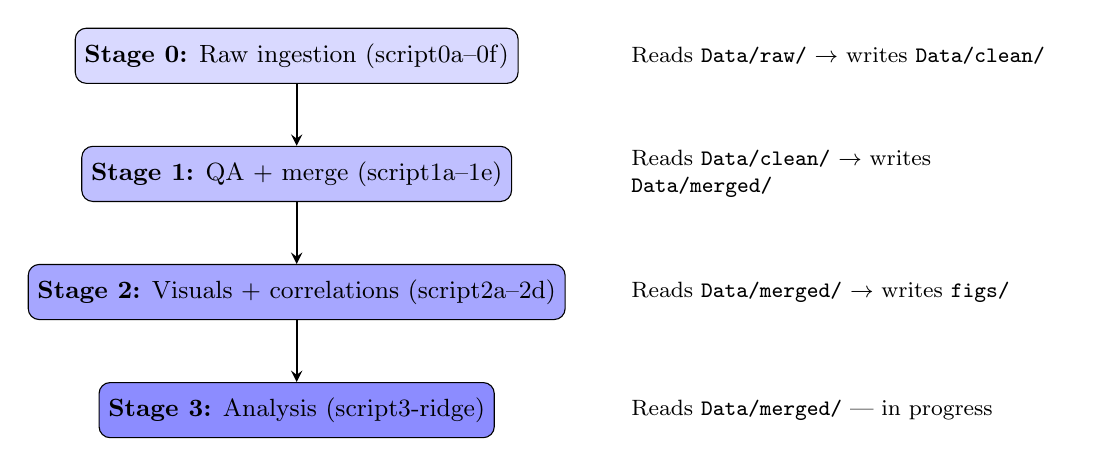
\begin{tikzpicture}[node distance=1.5cm, auto, font=\small]
  \node[draw, rounded corners, fill=blue!15, minimum width=3.5cm, minimum height=0.7cm] (s0) {\textbf{Stage 0:} Raw ingestion (script0a--0f)};
  \node[draw, rounded corners, fill=blue!25, minimum width=3.5cm, minimum height=0.7cm, below of=s0] (s1) {\textbf{Stage 1:} QA + merge (script1a--1e)};
  \node[draw, rounded corners, fill=blue!35, minimum width=3.5cm, minimum height=0.7cm, below of=s1] (s2) {\textbf{Stage 2:} Visuals + correlations (script2a--2d)};
  \node[draw, rounded corners, fill=blue!45, minimum width=3.5cm, minimum height=0.7cm, below of=s2] (s3) {\textbf{Stage 3:} Analysis (script3-ridge)};
  \draw[arrow] (s0) -- (s1);
  \draw[arrow] (s1) -- (s2);
  \draw[arrow] (s2) -- (s3);
  \node[right of=s0, xshift=5.5cm, text width=5.5cm, font=\footnotesize] {Reads \texttt{Data/raw/} $\rightarrow$ writes \texttt{Data/clean/}};
  \node[right of=s1, xshift=5.5cm, text width=5.5cm, font=\footnotesize] {Reads \texttt{Data/clean/} $\rightarrow$ writes \texttt{Data/merged/}};
  \node[right of=s2, xshift=5.5cm, text width=5.5cm, font=\footnotesize] {Reads \texttt{Data/merged/} $\rightarrow$ writes \texttt{figs/}};
  \node[right of=s3, xshift=5.5cm, text width=5.5cm, font=\footnotesize] {Reads \texttt{Data/merged/} — in progress};
\end{tikzpicture}
\end{center}
\vspace{0.3em}
{\footnotesize \textbf{Key utility files:} \texttt{packages.py} sets all shared imports and Dropbox path roots. \texttt{functions.py} provides FIPS normalization, CSV fallback readers, API wrappers, and the \texttt{latest\_files\_by\_descriptor()} selector used in Stage 1.}
\end{frame}

% ─────────────────────────────────────────────────────────────────────────────
%  SECTION 4: SOURCE-BY-SOURCE CLEANING DETAIL
% ─────────────────────────────────────────────────────────────────────────────

\begin{frame}{script0a: Population + FIPS Panel}
\textbf{Purpose:} Build a complete annual FIPS-year population panel from 1990--2024 using four Census vintages.

\vspace{0.5em}
\textbf{Inputs:} \texttt{Data/raw/population/*.csv} (4 Census files) and \texttt{Data/raw/fips/foruse\_*.txt} (pipe/comma/whitespace delimited crosswalks)

\vspace{0.5em}
\textbf{Key cleaning steps:}
\begin{enumerate}\small
    \item Reads each Census file by fragment name match (\texttt{cc-est2024}, \texttt{cc-est00int-tot}, etc.) — \textbf{if filenames change, these fragment strings must be updated}
    \item Identifies FIPS crosswalk delimiters via \texttt{sniff\_delimiter()} and reads accordingly (pipe / comma / fixed-width)
    \item Expands each decade's crosswalk to annual rows via \texttt{expand\_years\_cross()}
    \item \textbf{Hardcoded manual fix:} FIPS 12025 $\rightarrow$ 12086 (Miami-Dade) and two counties added for 1990 (Yellowstone NP \texttt{30113}, South Boston \texttt{51780})
    \item Drops state-level summary rows where \texttt{county == state}
    \item Normalizes DC to \texttt{11001}; drops non-US state codes; deduplicates on \texttt{(fips, year)} keeping last
\end{enumerate}

\vspace{0.3em}
\textbf{Output:} \texttt{Data/clean/YYYY-MM-DD\_population\_full.csv} — \textbf{100\% county-year coverage} used as the population denominator throughout the project.
\end{frame}

\begin{frame}{script0b: USDA NASS Agriculture (CAFO)}
\textbf{Purpose:} Pull CAFO operation counts by animal and size class from USDA NASS Quick Stats API (census years: 2002, 2007, 2012, 2017).

\vspace{0.3em}
\textbf{Key assumptions and hardcoded values:}
\begin{itemize}\small
    \item \textbf{API key:} \texttt{os.environ["USDA\_NASS\_API\_KEY"] = "30643212-..."} — \textbf{must be changed per user}
    \item \textbf{API fallback:} If API fails, reads \texttt{.dta} files from \texttt{Data/raw/usda/}
    \item \textbf{2012/2017 backfill:} Due to API failures, these years are backfilled from \texttt{donor\_path = ".../2026-02-23\_ag\_annual\_df.csv"} — \textbf{path must be updated if file moves}
    \item Filters to: \texttt{CENSUS} source, \texttt{COUNTY} level, animals = \{CATTLE, CHICKENS, HOGS\}, unit = \{HEAD, OPERATIONS\}
    \item Splits queries $>50{,}000$ rows by domain to avoid API limits (rate sleep: 0.4s)
\end{itemize}

\textbf{Size classification thresholds} (USDA CAFO definition, applied per inventory bin code):
\begin{tblr}{colspec={Q[l,2.5cm] Q[c,2cm] Q[c,2cm]}, hlines, vlines, row{1}={font=\bfseries\small}, row{2-Z}={font=\small}}
Animal & Medium $\geq$ bin & Large $\geq$ bin \\
Broiler chickens & 3 & 5 \\
Layer chickens & 7 & 9 \\
Cattle / Hogs & 6 & 7 \\
\end{tblr}

\vspace{0.3em}
\textbf{Outputs:} \texttt{*\_cafo\_ops\_by\_size\_compact.csv} (pivot: county $\times$ year $\times$ commodity $\times$ small/medium/large)
\end{frame}

\begin{frame}{script0c: Health Data (CHR + CDC Mortality)}
\textbf{Purpose:} Clean County Health Rankings (CHR) mental health surveys and CDC deaths-of-despair county files; merge into a single health panel.

\vspace{0.3em}
\textbf{CHR cleaning (Pass 1):}
\begin{itemize}\small
    \item Year inferred from filename via regex — \textbf{filenames must contain a 4-digit year}
    \item Column names normalized: lowercased, special characters stripped, label drift harmonized (e.g.\ \texttt{limited access to healthy foods} $\rightarrow$ \texttt{access to healthy foods})
    \item Duplicate columns resolved by keeping the most complete version (highest fill rate)
    \item \textbf{Variable selection thresholds:} include if present in $\geq 11$ annual files (majority rule) OR $\geq 8$ files with $\geq 80\%$ average fill
\end{itemize}

\textbf{CDC cleaning (Pass 2):}
\begin{itemize}\small
    \item Reads files matching \texttt{cty-level-deathsofdespair-YYYY.csv} from \texttt{Data/raw/cdc/}
    \item Parses: deaths, population, crude rate, \texttt{is\_unreliable} flag (from ``unreliable'' / ``suppressed'' in notes)
    \item \textbf{Suppression caveat:} crude rate is missing for \textasciitilde85--93\% of rural county-years (CDC suppresses when deaths $< 10$). Raw death count is always retained.
\end{itemize}

\textbf{Merge:} Outer join of CHR + CDC on \texttt{(fips, year)}; validated as 1:1. \\
\textbf{Outputs:} \texttt{*\_mentalhealthrank\_full.csv}, \texttt{*\_cdc\_county\_year\_deathsofdespair.csv}, \texttt{*\_mh\_mortality\_fips\_yr.csv}
\end{frame}

\begin{frame}{script0d: Crime Data (FBI UCR)}
\textbf{Purpose:} Stack annual FBI UCR incident files, select violent crime columns, collapse to FIPS-year counts.

\vspace{0.3em}
\textbf{Key steps:}
\begin{enumerate}\small
    \item Loads all \texttt{.csv} from \texttt{Data/raw/crime/total-v1/} (\textasciitilde 7 GB combined in memory — beware on low-RAM machines)
    \item \textbf{Crime types selected} by research team: aggravated assault, DUI, fondling, incest, intimidation, kidnapping, rape, sexual assault, simple assault, statutory rape, human trafficking (commercial sex + involuntary servitude)
    \item Column normalization: unicode dash normalization, whitespace collapse, then fuzzy matching for human trafficking columns (encoding issues required manual rename map)
    \item Collapses first to \texttt{(fips, year, sex, race, ethnicity)} keys, then \textbf{further to \texttt{(fips, year)} only} for the main panel
    \item \textbf{Optional disaggregation extension} (off by default): set env var \texttt{RUN\_CRIME\_DISAGG\_EXTENSION=1} to produce sex/age/race breakdowns in \texttt{interim-data/crime-disagg-extension/}
\end{enumerate}

\vspace{0.3em}
\textbf{Hardcoded paths:} \texttt{interim\_override} in script — update per user. \\
\textbf{Outputs:} \texttt{*\_crime\_fips\_level\_final.csv} (main), \texttt{*\_crime\_demog\_final.csv} (with demographics)
\end{frame}

\begin{frame}{script0e: NCHS Urban-Rural Classification}
\textbf{Purpose:} Build an annual rural/urban classification panel from the NCHS 6-level code scheme, used to define the analytical sample.

\vspace{0.3em}
\textbf{NCHS 6-level scheme:}
\begin{tblr}{colspec={Q[c,1.5cm] Q[l,4.5cm] Q[c,3cm]}, hlines, vlines, row{1}={font=\bfseries\small}, row{2-Z}={font=\small}}
Code & Label & non\_large\_metro \\
1 & Large central metro & \textbf{0 (excluded)} \\
2 & Large fringe metro & \textbf{0 (excluded)} \\
3 & Medium metro & 1 (included) \\
4 & Small metro & 1 (included) \\
5 & Micropolitan & 1 (included) \\
6 & Noncore (rural) & 1 (included) \\
\end{tblr}

\vspace{0.3em}
\textbf{Annual expansion logic:} NCHS provides codes at four base years (1990, 2006, 2013, 2023). Each base year is forward-filled to cover the next period:
\begin{itemize}\small
    \item 1990 code $\rightarrow$ 1990--2005; 2006 code $\rightarrow$ 2006--2012; 2013 code $\rightarrow$ 2013--2022; 2023 code $\rightarrow$ 2023
\end{itemize}

\textbf{Panel restricted to years $\geq$ 2000.} \\
\textbf{Output:} \texttt{YYYY-MM-DD-rural-key.csv} — the filter applied in \texttt{script1c}.
\end{frame}

\begin{frame}{script0f: FSIS Slaughterhouse Pipeline}
\textbf{Purpose:} Orchestrates a multi-step pipeline to clean FOIA-requested FSIS inspection data and recover FIPS codes via the HUD ZIP-to-FIPS crosswalk.

\vspace{0.3em}
\textbf{Pipeline sub-scripts (run in order):}
\begin{enumerate}\small
    \item \texttt{script0e-fsis-slaughterhouses.py} — extract raw FSIS inspection records
    \item \texttt{script0h-fsis-establishment-size-panel.py} — build establishment × size panel
    \item \textbf{HUD fill} (choose strategy via \texttt{--hud-strategy}):
    \begin{itemize}
        \item \texttt{bulk} (default): ZIP-to-FIPS crosswalk for all establishments with city/state/ZIP
        \item \texttt{targeted}: only missing establishments
        \item \texttt{skip}: no HUD fill
    \end{itemize}
    \item \texttt{script0l} — apply manual ZIP template (if present in \texttt{qa-fsis/})
    \item \texttt{script0m} — deterministic FIPS completion
    \item \texttt{script0n} — apply manual county labels (if present)
\end{enumerate}

\vspace{0.3em}
\textbf{Requirements:} \texttt{HUD\_API\_TOKEN} env var required (unless \texttt{--hud-strategy skip}). \\
\textbf{Coverage note:} FSIS data is \textbf{2017 only} — usable for cross-section analysis only, not panel. \\
\textbf{Output:} \texttt{*\_fsis\_county\_year\_fips\_est\_size\_type\_summary\_hudbulk\_manualzip.csv}
\end{frame}

% ─────────────────────────────────────────────────────────────────────────────
%  SECTION 5: MASTER MERGE (script1c)
% ─────────────────────────────────────────────────────────────────────────────

\begin{frame}{script1c: Master Merge — How It Works}
\textbf{Purpose:} Combine all clean source files into one county-year panel, restricted to rural counties.

\vspace{0.3em}
\textbf{Step-by-step logic:}
\begin{enumerate}\small
    \item \textbf{Auto-selects latest files} from \texttt{Data/clean/} by descriptor string (date prefix stripped)
    \item \textbf{Builds rural allowed-keys:} reads \texttt{*-rural-key.csv}, keeps only \texttt{(fips, year)} where \texttt{non\_large\_metro == 1}
    \item \textbf{Base panel:} CAFO compact file reduced to one row per \texttt{(fips, year)} — numeric columns summed (\texttt{min\_count=1} to preserve NaN for all-missing groups); text columns take first observed value
    \item \textbf{CAFO animal $\times$ size block:} pivot adds columns \texttt{cafo\_\{cattle/hogs/chickens\}\_\{small/medium/large\}}, \texttt{cafo\_total\_ops\_all\_animals}, \texttt{cafo\_total\_ops\_chickens}
    \item \textbf{Left-joins} CDC mortality, crime, FSIS, CHR mental health, and population onto the rural CAFO base
    \item \textbf{Derived crude rate:} \texttt{crude\_rate\_from\_census\_pop} = deaths / census population $\times$ 100{,}000 — computed only where deaths $> 0$ and population $> 0$
    \item \textbf{Missingness flags:} \texttt{cdc\_in\_query} (was county-year in CDC download?), \texttt{deaths\_is\_zero} (CDC returned 0 deaths — ambiguous, rate set to NaN)
\end{enumerate}
\end{frame}

\begin{frame}{script1c: Key Assumptions \& Caveats}
\begin{itemize}
    \item \textbf{Rural filter is the primary sample restriction.} Only counties coded \texttt{non\_large\_metro == 1} are in the panel. Large central and fringe metro counties are dropped entirely.
    \item \textbf{Column naming convention:} all merged columns are suffixed with the descriptor of their source file (e.g.\ \texttt{population\_population\_full}, \texttt{deaths\_cdc\_county\_year\_deathsofdespair}). Do not rename these manually.
    \item \textbf{Summing with \texttt{min\_count=1}:} When collapsing duplicates, numeric columns are summed but an all-missing group is preserved as NaN rather than coerced to 0.
    \item \textbf{Ambiguous CDC zeros:} \texttt{deaths\_is\_zero == 1} does not necessarily mean true zero deaths — could be suppression artefact. The crude rate is set to NaN for these rows. Do not treat them as confirmed no-death counties.
    \item \textbf{FSIS joins on year = 2017 only:} FSIS establishments appear only for 2017. All other years will have NaN in FSIS columns — this is expected.
    \item \textbf{Text column resolution:} String columns from multi-row sources take the \textit{first} non-null observed value after the rural filter. This is appropriate for geographic labels but should not be used for time-varying text fields.
\end{itemize}
\end{frame}

% ─────────────────────────────────────────────────────────────────────────────
%  SECTION 6: DERIVED VARIABLES & QA (script1d, script1e)
% ─────────────────────────────────────────────────────────────────────────────

\begin{frame}{script1e: Derived Variables (CHR Counts + Ratio Flags)}
\textbf{Purpose:} Two-pass augmentation of the merged panel using County Health Rankings data.

\vspace{0.5em}
\textbf{Pass 1 — Impute counts for rate-only CHR variables:}
\begin{itemize}\small
    \item Applies to 6 variables that have \texttt{raw\_value} only (no numerator column): frequent mental distress, frequent physical distress, insufficient sleep, access to exercise, \% American Indian/Alaskan Native, \% non-Hispanic African American
    \item Formula: \texttt{count\_imputed = (raw\_value / 100) $\times$ census\_population}
    \item Scale auto-detected: median $\leq 1$ $\Rightarrow$ proportion (multiply by 100); otherwise already a percentage
    \item \textbf{These are imputed, not measured counts.} Label: \texttt{*\_count\_imputed}
\end{itemize}

\vspace{0.3em}
\textbf{Pass 2 — Verify numerator/denominator consistency:}
\begin{itemize}\small
    \item For all CHR variables with both \texttt{numerator} and \texttt{denominator} columns, checks: \texttt{numerator / denominator $\approx$ raw\_value}
    \item Tolerance: absolute diff $>$ 0.05 (5 pp) OR relative diff $>$ 10\% $\Rightarrow$ flagged
    \item Flag column: \texttt{*\_ratio\_flag = 1}. Variables with $>5\%$ rows flagged generate a warning.
    \item \textbf{No values are modified} — flags only. Inspect flagged variables before use in regression.
\end{itemize}

\textbf{Output:} \texttt{*\_full\_merged\_derived.csv} (original panel unchanged)
\end{frame}

\begin{frame}{script1d: CDC Crude Rate Sense Check}
\textbf{Purpose:} Validate that CDC-reported crude rates align with rates recomputed from merged deaths + census population. Flags systematic discrepancies.

\vspace{0.3em}
\textbf{Diagnostics produced:}
\begin{itemize}\small
    \item \texttt{crude\_rate\_recalc\_census\_pop} = deaths / census pop $\times$ 100{,}000 (recomputed)
    \item \texttt{crude\_rate\_recalc\_cdc\_pop} = deaths / CDC pop $\times$ 100{,}000 (internal check)
    \item \texttt{diff\_census\_minus\_cdc}: difference between recomputed and CDC-reported rates
    \item \texttt{z\_diff\_from\_zero\_sd}: standardized distance of discrepancy from zero
    \item \texttt{population\_pct\_diff\_census\_vs\_cdc}: \% difference between Census and CDC population denominators
\end{itemize}

\vspace{0.3em}
\textbf{QA outputs} (saved to \texttt{Data/merged/figs/panel-sumstats-by-farms/}):
\begin{itemize}\small
    \item \texttt{*\_qa\_cdc\_cruderate\_sensecheck\_overall.csv} — global summary statistics
    \item \texttt{*\_qa\_cdc\_cruderate\_sensecheck\_by\_year.csv} — year-by-year breakdown
    \item \texttt{*\_qa\_cdc\_cruderate\_sensecheck\_outliers\_top1000.csv} — largest discrepancies
\end{itemize}

\vspace{0.3em}
{\small \textbf{Hardcoded paths in this script:} \texttt{MERGED\_DIR} and \texttt{OUT\_QA\_DIR} are absolute paths — update before running on a new machine.}
\end{frame}

% ─────────────────────────────────────────────────────────────────────────────
%  SECTION 7: THE FINAL MERGED PANEL
% ─────────────────────────────────────────────────────────────────────────────

\begin{frame}{The Final Merged Panel: What It Is}
\textbf{File:} \texttt{Data/merged/YYYY-MM-DD\_full\_merged.csv}

\vspace{0.5em}
\begin{columns}[T]
\column{0.48\textwidth}
\textbf{Unit of observation:} county-year (\texttt{fips}, \texttt{year})

\textbf{Sample restriction:} non-large-metro counties only (\texttt{non\_large\_metro == 1})

\textbf{Year range:} \textasciitilde2000--2022 (source-dependent)

\textbf{Panel structure:} unbalanced — not all sources cover all years

\textbf{Key identifier columns:}
\begin{itemize}\small
    \item \texttt{fips} — 5-digit zero-padded county FIPS
    \item \texttt{year} — integer year
    \item \texttt{non\_large\_metro} — always = 1 in this panel
\end{itemize}

\column{0.48\textwidth}
\textbf{Column naming convention:}

All non-key columns are suffixed with their source descriptor:
\begin{itemize}\small
    \item \texttt{..\_cafo\_ops\_by\_size\_compact} — CAFO columns
    \item \texttt{..\_cdc\_county\_year\_deathsofdespair} — CDC mortality
    \item \texttt{..\_mentalhealthrank\_full} — CHR survey
    \item \texttt{..\_crime\_fips\_level\_final} — UCR crime
    \item \texttt{..\_fsis\_county\_year\_..\_summary\_..} — FSIS plants
    \item \texttt{..\_population\_full} — Census population
\end{itemize}
\end{columns}
\end{frame}

\begin{frame}{The Final Merged Panel: Key Variables}
\begin{tblr}{
  colspec = {Q[l,3.5cm] Q[l,5cm] Q[l,3.5cm]},
  hlines, vlines,
  row{1} = {font=\bfseries\small},
  row{2-Z} = {font=\footnotesize},
}
Variable & Description & Source \\
\texttt{cafo\_\{animal\}\_\{size\}} & Count of small/medium/large CAFO ops by animal type (cattle, hogs, chickens) & USDA NASS census years \\
\texttt{cafo\_total\_ops\_all\_animals} & Total CAFO operations across all animal types & Derived in script1c \\
\texttt{population\_population\_full} & Annual county population (Census) & script0a — 100\% coverage \\
\texttt{deaths\_cdc\_...} & Raw deaths-of-despair count & CDC WONDER \\
\texttt{crude\_rate\_cdc\_...} & CDC-reported crude rate (suppressed $<10$ deaths) & CDC WONDER \\
\texttt{crude\_rate\_from\_census\_pop} & Recomputed crude rate using Census pop denominator & Derived in script1c \\
\texttt{cdc\_in\_query} & 1 if county-year appeared in CDC WONDER download & Derived flag \\
\texttt{deaths\_is\_zero} & 1 if CDC returned Deaths=0 (ambiguous) & Derived flag \\
\texttt{poor\_mental\_health\_days\_raw\_value\_...} & Avg days/month of poor mental health (CHR) & County Health Rankings \\
\texttt{frequent\_mental\_distress\_raw\_value\_...} & \% adults with frequent mental distress (CHR) & County Health Rankings \\
\texttt{n\_unique\_establishments\_fsis\_...} & Count of FSIS-regulated plants per county (2017 only) & USDA FSIS FOIA \\
\texttt{aggravated\_assault\_crime\_...} & UCR aggravated assault count & FBI UCR \\
\end{tblr}
\end{frame}

\begin{frame}{The Final Merged Panel: Coverage by Source}
\begin{tblr}{
  colspec = {Q[l,4cm] Q[c,2.5cm] Q[c,2.5cm] Q[l,3cm]},
  hlines, vlines,
  row{1} = {font=\bfseries\small},
  row{2-Z} = {font=\small},
}
Source & Year range & Fill (\% panel) & Notes \\
Census population & 1990--2024 & $\approx$ 100\% & Used as denominator \\
CAFO operations & 2002, 2007, 2012, 2017 & $\approx$ 97\% (census yrs) & Census years only \\
CHR poor mental health days & 2004--2022 & $\approx$ 90\% (2010+) & Usable 2010 onward \\
CHR frequent mental distress & 2016--2022 & $\approx$ 90\% (2016+) & Not for pre-2016 panel \\
CHR excessive drinking & 2011--2022 & $\approx$ 80\% (2011+) & Full from 2016 \\
CDC deaths of despair (raw count) & 1999--2020 & Varies & Count retained always \\
CDC crude rate & 1999--2020 & $<$ 15\% & Suppressed $<10$ deaths \\
FBI UCR crime & \textasciitilde 2000--2022 & Varies by year & Violent crime subset \\
FSIS establishments & \textbf{2017 only} & 2017 cross-section & Cross-section use only \\
\end{tblr}

\vspace{0.5em}
{\footnotesize \textbf{Recommended panel window for outcome analysis: 2010--2015.} This balances CHR mental health coverage ($\approx$90\%), CAFO census year availability (2012), and pre-FSIS comparability.}
\end{frame}

\begin{frame}{The Final Merged Panel: Data Quality Flags}
\textbf{Known issues and how to handle them:}

\vspace{0.5em}
\begin{enumerate}
    \item \textbf{CDC crude rate missingness ($\approx$85--93\%):} This is by design — CDC suppresses for $<10$ deaths. Use raw death counts or the recomputed \texttt{crude\_rate\_from\_census\_pop} for analysis. Flag \texttt{cdc\_in\_query = 0} means the county-year was absent from the CDC WONDER pull entirely (unknown true value).

    \item \textbf{FSIS data is 2017 cross-section only:} All panel years outside 2017 will be NaN in FSIS columns. Do not interpret as ``zero plants.'' Use a binary indicator or restrict to 2017.

    \item \textbf{CAFO data at census years only (2002, 2007, 2012, 2017):} Interpolating between census years is not recommended without strong justification — agricultural structure changes slowly but not uniformly.

    \item \textbf{CHR \texttt{frequent\_mental\_distress} starts 2016:} Cannot be used in a pre-2016 panel. Use \texttt{poor\_mental\_health\_days} (available from \textasciitilde 2004, reliable from 2010) as the primary mental health outcome for longer panels.

    \item \textbf{CAFO per-capita transformation:} Raw CAFO operation counts are heavily right-skewed. For scatter plots and regressions, use \texttt{log(cafo\_total\_ops\_all\_animals / population $\times$ 10{,}000 + 1)}.
\end{enumerate}
\end{frame}

\begin{frame}{The Final Merged Panel: Exported Slices}
\begin{tblr}{
  colspec = {Q[l,5cm] Q[l,4cm] Q[l,3cm]},
  hlines, vlines,
  row{1} = {font=\bfseries\small},
  row{2-Z} = {font=\small},
}
File suffix & Year range & Recommended use \\
\texttt{\_full\_merged.csv} & All years (rural) & Starting point for all analysis \\
\texttt{\_full\_merged\_2005\_2010.csv} & 2005--2010 & Pre-recession window \\
\texttt{\_full\_merged\_2010\_2020.csv} & 2010--2020 & \textbf{Recommended primary panel} \\
\texttt{\_full\_merged\_census\_years.csv} & 2002, 2005, 2007, 2012 & CAFO-aligned cross-sections \\
\texttt{\_full\_merged\_derived.csv} & All years + derived & CHR imputed counts + ratio flags \\
\end{tblr}

\vspace{0.5em}
\textbf{How to load the latest panel in Python:}
\begin{lstlisting}
from functions import latest_file_glob
import pandas as pd

merged_dir = "~/Dropbox/Mental/Data/merged"
path = latest_file_glob(merged_dir, "*_full_merged.csv")
df = pd.read_csv(path, low_memory=False)
# Always normalize the key after loading:
from functions import normalize_panel_key
df = normalize_panel_key(df, dropna=True)
\end{lstlisting}
\end{frame}

% ─────────────────────────────────────────────────────────────────────────────
%  SECTION 8: HARDCODED PATHS REFERENCE
% ─────────────────────────────────────────────────────────────────────────────

\begin{frame}{Hardcoded Paths: What Must Change Per User}
\textbf{Before running any script on a new machine, update the following:}

\vspace{0.5em}
\begin{tblr}{
  colspec = {Q[l,3cm] Q[l,5cm] Q[l,4cm]},
  hlines, vlines,
  row{1} = {font=\bfseries\small},
  row{2-Z} = {font=\footnotesize},
}
Script & Variable / Line & What to change \\
\texttt{packages.py} & \texttt{db\_base = os.path.expanduser("$\sim$/Dropbox/Mental")} & Dropbox root path \\
\texttt{script0a, 0b, 0d} & \texttt{repo = "/Users/allegrasaggese/Documents/..."} & GitHub repo path \\
\texttt{script0b} & \texttt{USDA\_NASS\_API\_KEY} env var & Personal API key \\
\texttt{script0b} & \texttt{donor\_path = ".../2026-02-23\_ag\_annual\_df.csv"} & Backfill CSV path \\
\texttt{script0d} & \texttt{interim\_override = "/Users/allegrasaggese/Dropbox/..."} & Local Dropbox copy path \\
\texttt{script0f} & \texttt{HUD\_API\_TOKEN} env var & HUD API token \\
\texttt{script1d} & \texttt{MERGED\_DIR}, \texttt{OUT\_QA\_DIR} & Absolute output paths \\
\end{tblr}

\vspace{0.5em}
{\footnotesize \textbf{Best practice:} Set \texttt{db\_base} in \texttt{packages.py} to the correct Dropbox root for your machine. All other paths are derived from \texttt{db\_base} via \texttt{os.path.join()} and will resolve automatically once this is set correctly.}
\end{frame}

\end{document}
